\documentclass[12pt,fleqn]{article}\usepackage{../common}
\begin{document}
Filtrelemek

Filtreler dis dunyadaki bir aksiyon hakkinda elde edilen gurultulu
sinyalleri, tersine cevirerek arka plandaki aksiyon hakkinda hesaplama
yapabilmemizi saglar. Mesela Kalman Filtreleri (KF) icin gizlenmis konum
bir robotun nerede oldugu, bir senetin fiyati gibi bir sey olabilir, gizli
konum bilgisi $x_t$ degiskeninde o konum hakkindaki gurultulu olcum $y_t$
icindedir. Hem gizli konumlar arasindaki gecis, hem de olcumun gurultusu
lineer bir fonksiyon uzerindendir.

\[ x_{t+1} = Ax_t + v \]

\[ y_t = Hx_t + w \]

$v$ ve $w$'in dagilimi Gaussian'dir ve kovaryans sirasiyla $Q$ ve $R$
icindedir. 

Zaman faktorunu de dahil etmek gerekirse;

\[ \hat{x}_t^t = E[x_t|y_0,..,y_t] \]

\[ P_t^t = E[(x_t - \hat{x}_{t|t}) (x_t - \hat{x}_{t|t})'| y_0,...,y_t   ] \]

Filtremenin amaci $x_{t+1}$ ve $P_{t+1}$ hesabini yeni bir olcum $y_{t+1}$
uzerinden yapmak olacak. ``Gizli'' $x_t$ derken bunu kastediyorduk, bu
deger bize verilmiyor, sadece xt ve $x_{t+1}$ arasindaki gecisin nasil oldugunu
biliyoruz, gurultunun nasil eklendigini biliyoruz, ama bunlarin bilsek bile
elde bir suru bilinmeyen var. Filtrelemenin matematiksel numaralari
sayesinde bunu hesaplayabiliyor olacagiz.  Yani yapmamiz gereken ``oku
tersine cevirmek'', yani $x_t$'nin $y_t$ uzerindeki sartsal bagliligini
(conditional dependence) ortaya cikartmak, bunu $y_t$'nin $x_t$'ye olan sartsal
bagimliligini tersine cevirerek yapmak. Ana denklemin iki tarafinin da
beklentisini (expectation) alalim:

\[ E \ x_{t+1} = \hat{x}_{t+1} = A \mu_t = A \hat{x}_t \]

Simdi iki tarafin kovaryansini alalim ve $P_t$'yi $cov \ x(t)$ olarak
belirtelim:

\[ P_{t+1} = AP_tA' + Q \]

Bu gecis ``zaman guncellemesi'' olarak adlandirilir. Normal dagilimlari $t$
anindan $t + 1$ anina gecirmemizi saglar. $y$ iceren formullerde benzer bir
durum var. 

\[ \hat{x}_{t+1}^t = Ax_t^t \]

\[ P_{t+1}^t = AP_t^tA' + Q \]

\[ y_{t+1} = Cx_{t+1} + w_t \]

\[ E[y_{t+1}|y_0,..,y_t] = E[Cx_{t+1} + w_t | y_0,..,y_t] \]

\[ \hat{y}_{t+1}^t = C\hat{x}_{t+1} \]

Kovaryans icin benzer durum

\[ E[(y_{t+1}-\hat{y}_{t+1}^t)(y_{t+1}-\hat{y}_{t+1}^t)' | y_0,...,y_t] = 
C_{t+1}^t C' + R
 \]

 Simdi daha zor is olan oku tersini cevirmeye gelelim. Eger amacimiz p(xt
 |yt ) denklemini elde etmek ise o zaman bu iki degiskeni iceren birlesik
 dagilimi (joint distribution) elde etmek zorundayiz. Iki Gaussian'in
 birlesiminin yeni bir Gaussian oldugunu biliyoruz, o zaman hem $x_t$ hem
 de $y_t$'in kendisi cok boyutlu birer Gaussian olduklari icin onlarin
 birlesimi $p(x_t |y_t )$'in hakikaten devasa bir Gaussian olacagini tahmin
 edebiliriz.

$x_t$ ve $y_t$'in birlesimi olan Gaussian'i bulmak demek, bu Gaussian'in 
ortalamasini (mean) ve kovaryansini bulmak demektir cunku bir Gaussian 
ortalama ve kovaryansi ile net bir sekilde tanimlanabilir bir seydir. 
Bir numara yapalim, ve $y_t = Cx_t + w_t$'yi $z = Hu$ seklinde
yazalim. Sonra 

\[ 
\left[\begin{array}{r}
x_t \\
y_t
\end{array}\right], 
H = 
\left[\begin{array}{rr}
I & 0 \\
C & I
\end{array}\right], 
u = 
\left[\begin{array}{r}
x_t \\
w_t
\end{array}\right]
 \]

Boylece daha basit bir denklemin kovaryansini alabiliriz

\[ cov(z) = H \cos(u) H' \]

\[ 
cov(u) = 
\left[\begin{array}{rr}
P_t & 0 \\
0 & R
\end{array}\right]
 \]

Tam carpim suna esit

\[ 
\left[\begin{array}{rr}
I & 0 \\
C & I
\end{array}\right]
\left[\begin{array}{rr}
P_t & 0 \\
0 & R
\end{array}\right]
\left[\begin{array}{rr}
I & C' \\
0 & I
\end{array}\right]
 \]

bunun sonucu ise

\[ 
\left[\begin{array}{rr}
P_t & P_t C' \\
CP_t & CP_tC' + R
\end{array}\right]
 \]

Bunu baglantisal denklem icin ve ortalamayi icerecek sekilde yazabiliriz

\[ 
\left[\begin{array}{r}
\hat{x}_t^t \\
C\hat{x}_t^t
\end{array}\right] 
, 
\left[\begin{array}{rr}
P_t^t & P_t^tC' \\
CP_t^t & CP_t^t + R
\end{array}\right]
 \]

Ayni sekilde $x_{t+1} , y_{t+1}$ birlesik dagilim icin

\begin{equation}\label{eq1}
\left[\begin{array}{r}
\hat{x}_{t+1}^t \\
C\hat{x}_{t+1}^t
\end{array}\right], 
\left[\begin{array}{rr}
P_{t+1}^t & P_{t+1}^tC' \\
CP_{t+1}^t & CP_{t+1}^tC' + R
\end{array}\right]
\end{equation}

Simdi $x_{t+1}^{t+1}$ 'in ortalama ve varyansi icin parcali Gaussian kavramini
anlatmaliyiz. Bir n boyutlu Gaussian daha kucuk boyutlardaki p ve q alt
Gaussian'lara parcalanabilir (tabii ki $n = p + q$). Yani su ifade
kullanilabilir

\begin{equation}\label{eq2}
\mu = 
\left[\begin{array}{r}
\mu_1 \\ \mu_2
\end{array}\right], 
\Sigma = 
\left[\begin{array}{rr}
\Sigma_{11} & \Sigma_{12} \\
\Sigma_{21} & \Sigma_{22} 
\end{array}\right]
\end{equation}

\[ 
p(x|\mu,\Sigma) = 
\frac{1}{(2\pi)^{(p+q)/2}|\Sigma|^{1/2}}
exp \bigg\{ 
-\frac{1}{2} 
\left(\begin{array}{rr}
x_1 - \mu_1 \\
x_2 - \mu_2 
\end{array}\right)'
\left[\begin{array}{rr}
\Sigma_{11} & \Sigma_{12} \\
\Sigma_{21} & \Sigma_{22} 
\end{array}\right]^{-1}
\left(\begin{array}{rr}
x_1 - \mu_1 \\
x_2 - \mu_2 
\end{array}\right)
\bigg\}
 \]

Uzun cebirsel islemlerden sonra $p(x_1|x_2)$ ifadesini elde ederiz. Bu
cebirsel turetimi gormek istiyorsaniz, {\em Istatistik} ders notlarimizda
Ders 3'e bakabilirsiniz.

Bundan sonra sartlanmis (conditioned) $\mu$ ve $\Sigma$ alinir.

\begin{equation}\label{eq3}
\mu_{1|2} = \mu_1 + \Sigma_{12}\Sigma_{22}^{-1}(x_2 - \mu_2) 
\end{equation}

\[ \Sigma_{1|2} = \Sigma_{11}- \Sigma_{12}\Sigma_{22}^{-1}\Sigma_{21} \]

Simdi denklem \ref{eq3}'u alip \ref{eq1}'in icine koydugumuzda ve
\ref{eq2}'deki yerlesim yapisini dikkate aldigimizda $\hat{x}_{t+1}^{t+1}$
ve $P_{t+1}^{t+1}$ formullerini ortaya cikartabiliriz. 

\[ \hat{x}_{t+1}^{t+1} =  x_{t+1}^{t} +  P_{t+1}^{t}C'(CP_{t+1}^{t}C' + \Sigma_w)^{-1}
(y_{t+1}- C\hat{x}_{t+1}^t)
\]

\[ P_{t+1}^{t+1} = P_{t+1}^{t} - P_{t+1}^{t} C'(CP_{t+1}^{t} C'+R)^{-1}CP_{t+1}^{t} 
\]

Eger $K = P_{t+1}^{t}C'(CP_{t+1}^{t}C' + \Sigma_w)^{-1}$ dersek

\[  \hat{x}_{t+1}^{t+1}  =  \hat{x}_{t+1}^{t} + K_t (y_{t+1} - C \hat{x}_{t+1}^{t}  \]

\[  P_{t+1}^{t+1} =  P_{t+1}^{t} - K_tC P_{t+1}^{t} \]

Ornek: Veriye Duz Cizgi Uydurmak (Line Fitting)

Eger elimizde bir cizgiye uydurmak icin kullanacagimiz tum veri olsaydi,
uydurma islemi icin en az kareler (least sqaures) yontemini
kullanabilirdik.  Kalman Filtreleri bize yeni veri geldigi anda, her
seferinde, azar azar bir cizgiyi uydurmamizi sagliyor. Hatta matematiksel
olarak ispalanmistir ki eger baslangic noktasi ayniysa, azar azar veriyi KF
ile almanin sonunda, tum veriyi bir kerede en az karesel yontem ile
uydurmak ayni sonucu verir.

Peki bu uydurma islemini nasil yapariz? Burada veriyi nasil temsil ettigimiz
konusunda ufak bir numara kullanmamiz lazim.

Kendimize bir soru soralim: bu sistemin konum bilgisi nedir? Bir robotu
izliyorsak mesela soru cevabi basittir, onun $x, y$ gibi kordinat
bilgisi. Duz cizgi fit ederken takip edilen bunlar degil, bize gerekli olan
bir cizginin ``egimi (slope)''. Yani hem bir cizginin y eksenini kestigi
nokta, hem de cizginin egimi xt konum bilgisi icinde dahil edilecek. Burada
KF literaturunden gelen $x, y$ harfleri birbirine karismasin diye cizginin
degerlerini $xx_t$ ve $yy_t$ olarak tanimlayacagiz. O zaman $x_t$ vektoru suna
benzer:

\[ x_t = 
\left[\begin{array}{r}
yy_t \\
a
\end{array}\right]
 \]

ki burada $a$ harfi egimi temsil etmektedir. $a$ bir sabit olduguna gore
KF her zaman diliminde ayni kalacak bir degiskeni
hesaplayacaktir. Cogunlukla KF ile her zaman diliminde degisik olan
degerlerin hesaplandigini goruruz, bu uygulamaya gore degisen bir seydir,
matematiksel bir mecburiyet degildir. $A$ matrisimiz ile de biraz numara
yapmamiz gerekli. Bu matris $x_t$'yi donusturup $x_{t+1}$'i elde etmemizi
saglayan sey olduguna gore $A$'nin soyle olmasi gerekir:

\[ 
A_t = 
\left[\begin{array}{rr}
1 & \Delta xx \\
0 & 1
\end{array}\right]
 \]

Bu matrisi $x_t$ ile carptigimizda $yy_t \cdot 1 + a \cdot \Delta xx$
degerini elde ediyoruz, ki bu deger bir cizgi uzerinde bir sonraki noktayi
temsil ediyor. Dis olcumu veren gurultu matrisi $H$ ise

\[ H =
\left[\begin{array}{rr}
1 & 0 \\
1 & 0
\end{array}\right]
 \]

seklinde. Bunu $x_t$ ile carptigimizda $y_t$'yi (iki kere) elde ettigimizi
gorecegiz.  Not: Niye iki kere? Kodlama sirasinda boyutlarin uyumlu olmasi
icin boyle gerekti, cok buyuk bir rahatsizlik degil. Kod altta
gorulebilir.

\lstinputlisting[language=Python]{kalman_slope.py}

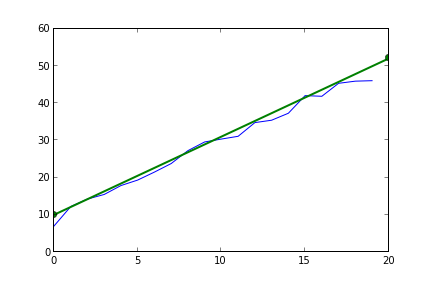
\includegraphics[height=7cm]{kalman-line-fit.png}

Ornek: Obje Takibi

Daha degisik bir ornekten bahsedelim. Bu ornekte OpenCV kutuphanesinden
elde ettigimiz 2 boyutlu degerleri $y_t$ icin kullanacagiz. Degerler
OpenCV'nin bir satranc tahtasi seklinin kose noktalarini otomatik olarak
bulabilen cvFindChessboardCorners cagrisinden gelecek (ayrica
cvDrawChessboardCorners ile bu noktalari ekranda aninda gosterebilecegiz).

Elimizdeki ``gurultulu'' olcumler iki boyutlu noktasal degerler. Gurultulu
cunku kamera bize bu imajlari aktarirken hata eklemis olabilir, OpenCV
fonksiyonu hesabi yaparken hata eklemis olabilir, bir suru olasilik var.

Bu ornekte, ayrica, ilk kez KF ortaminda boyut degisikligi olasiligini net
bir sekilde gorebiliyoruz. Gizli konum bilgisi $x_t$ 3 boyutlu bir nokta,
ama elimizdeki olcum 2 boyutlu bir ``yansima''. Yansima sirasinda
kacinilmaz olarak deger kaybediliyor, bir boyutun bilgisi ortadan
yokoluyor. Ama tum bu bilinmezlere ragmen Kalman filtresinin bizim icin
gizli bilgiyi hesaplamasini istiyoruz.

Bu problemde A matrisi ne olacaktir? Obje takibi konularinda A'nin ne
oldugunu hayal etmek daha kolay, A matrisi iki zaman dilimi arasindaki
``hareketi'' temsil edecek. Bu problemdeki ek bir kolaylik bu hareketi
onceden bildigimiz, ve hareketin tek yonde oldugu. Yani resimde benim
tuttugum kartonu ne kadar hizla hareket ettirdigimi ben onceden probleme
bildiriyorum. Yer degisikligini $d$ olarak betimledim, ve $A$ soyle oldu:

\[ A = 
\left[\begin{array}{rrrr}
1 & 0 & 0 & 0 \\
0 & 1 & 0 & 0 \\
0 & 0 & 1 & d \\
0 & 0 & 0 & 1
\end{array}\right]
 \]

Dikkat edersek $A$ 4x4 boyutunda, 3x3 degil. 3 boyutlu kordinatlari temsil
etmek icin homojen kordinat sistemini kullandigimiz icin boyle oldu, o
sebe- ple zaten $x_t$ de 4x1 oldu, ona uymak icin $A$'nin degismesi
gerekiyordu. $Ax_t$ carpiminin hakikaten kartonu hareket ettirdigini
gostermek icin bu carpimi bir ornek uzerinde yapalim: Diyelim 
ki $x_t = [
 a_1 \ a_2 \ a_3 \ a_4 ]$ o zaman $Ax_t$ ya da $x_{t+1}$ su hale gelir: $[
 a_1 \ a_2 \ a_3+d \ a_4 ]$.

Bakiyoruz, hakikaten de d kadarlik bir yer degisimi z kordinati, yani
derinlik uzerinde eklenmis. Test amaclarimiz icin d = -0.5 aldik, yani
satranc tahta kartonunun her zaman diliminde kameraya dogru 0.5 cm
ilerledigini belirttik. Tabii bu da kabaca bir tahmindi (her ne kadar
hareketi yaptiran ben olsam bile!), ama filrelemenin gucunu burada
goruyoruz. Benim tahminimde ``gurultu'' yani ``hata payi'' var, olcumde
gurultu var, tum bunlar ust uste konsa bile filtre yine de gizli konumu
bulacak.

Olcumsel donusumu temsil eden H'e ben onun temeli olan yansima (projection)
kelimesinden gelen P matrisinden bahsedelim. Yansima matrisi goruntu
(vision) literaturunde tek delikli kamera (pinhole camera) modelinden ileri
gelen bir matristir ve bu matrisi hesaplamak ayarlama / kalibrasyon
(calibration) denen apayri bir islemin parcasidir. OpenCV icinde
kalibrasyon icin fonksiyonlar var, biz de bunlari denedik, kalibrasyon icin
kullandigimiz resimlerle alakali olmali, elde edilen sonuclardan memnun
kalmadik. Alternatif olarak sunu yaptik; resimde gorulen yesil yuzey bizim
programin olustur- dugu hayali bir yuzey. Filtrenin o anki tahminini P
uzerinden goruntuye yansitarak bu yuzeyi olusturduk, boylece deneme /
yanilma yontemiyle pek cok P degerini deneyerek, yuzeyin resimde gorulen
masanin sonunda cikacak sekilde olmasini sagladik. O noktaya gelince
istedigimiz P degerini bulmus oluyorduk. Yansitma matrisleri 3x3 olur, KF
buna bir dorduncu [0 0 0] satiri ekleyerek onu 4x3 H haline getiriyor.

KF'in baslangic noktasi olarak P'yi bulmak icin kullandigimiz masa sonunu
kullandik. Kararsizlik olcutu Q icin, ki bu degisken bir Gaussian kovaryan-
sidir, $Q = I \cdot 150 cm$ degerini kullandik, yani oldukca buyuk bir
kararsizlik degeri kullandik. Sebep baslangic degeri olan masa ortasini
sectik, ve takip edecegimiz satranc tahtasinin nerede oldugunu bilmiyoruz,
``emin degiliz''.  Bu kararsizligi sayisal olarak programa bildirmis olduk.

Alttaki resimlerde filtrenin tahminini temsil eden yesil yuzeyin satranc tah-
tasini basariyla takip ettigini goreceksiniz.

\lstinputlisting[language=Python]{kalman_3d.py}

\lstinputlisting[language=Python]{track-chess-kf.py}

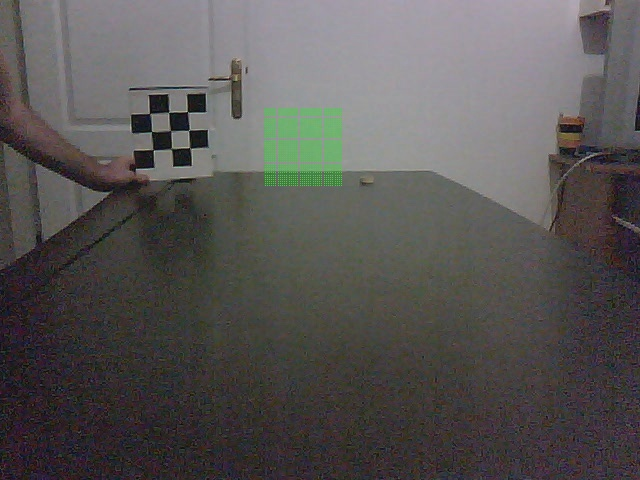
\includegraphics[height=4cm]{cb-kf-00.jpg}

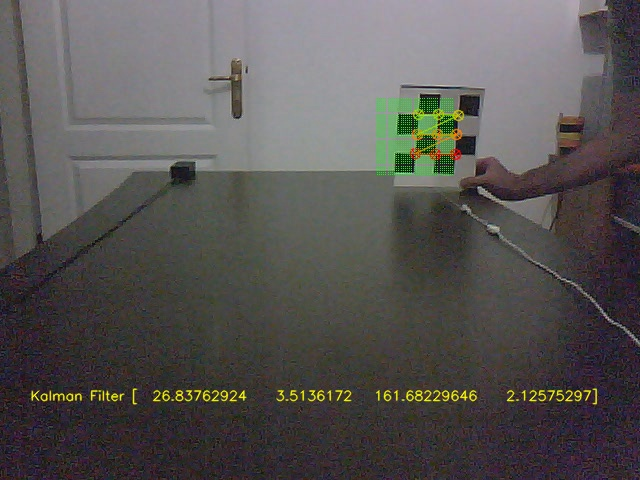
\includegraphics[height=4cm]{cb-kf-1.jpg}

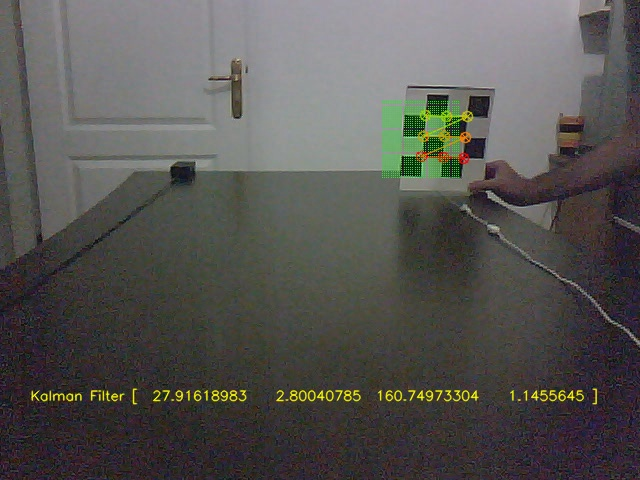
\includegraphics[height=4cm]{cb-kf-2.jpg}

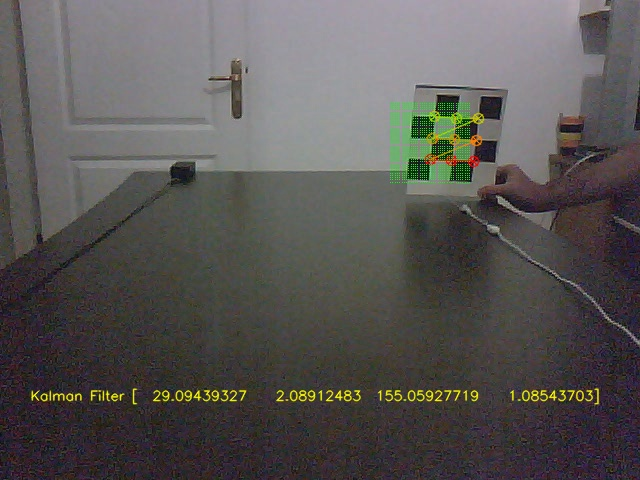
\includegraphics[height=4cm]{cb-kf-3.jpg}

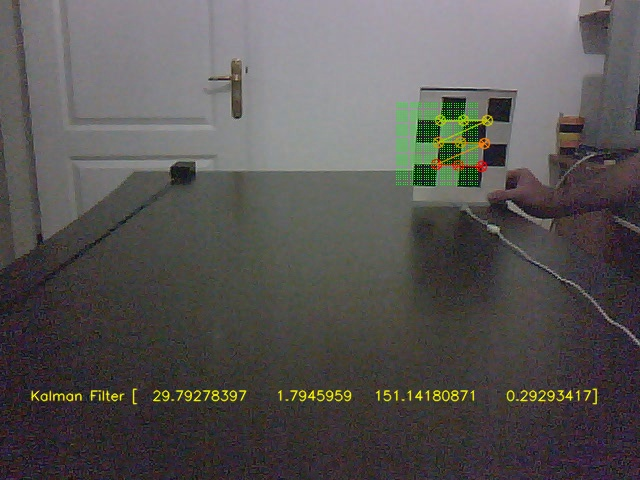
\includegraphics[height=4cm]{cb-kf-4.jpg}

Parcacik Filtreleri

Filtrelemede tek yontem Kalman filtreleri degil. KF kararsizlik Gaussian
olarak gosterilebiliyorsa cok faydali, ve hizli bir yontem. Bir KF bellekte
cok az yer tutar, 3 boyutlu bir Gaussian icin 3x1 boyutunda bir ortalama
vektoru, ve 3x3 boyutunda bir kovaryans matrisi yeterlidir, yani 3 + 9 = 12
sayi.

Parcacik filtreleri (PF) bir dagilimi ``ayriksal'' olarak temsil
ederler. Yani diyelim ki tek boyutlu bir dagilimi 100 eleman iceren bir
dizin ile temsil ede- biliriz, o zaman dagilimin degerlerini 100 tane
noktada tasimamiz gerekir.  Bunun faydalari her turlu dagilim seklini
temsil edebilmemiz. Gaussian sadece belli bir sekilde olabilir, tek bir
tepe noktasi olmalidir, vs. Ayriksal temsil ile 2, 3, istedigimiz kadar
tepe noktasi olan (ya da hic olmayan) bir dagilim kullanabiliriz.

Bu neye yarar? Birden fazla hipotezi ayni anda isletebilmemize yarar. KF
ile tepe noktasi en iyi tahminimizdir (mesela.. satranc kartonu masa
ortasinda), PF ile birkac tahmini ayni anda hesaplatmak mumkun olabilir.

Daha detaylandirmak gerekirse, PF kodlamasi $x_t$ icin iki tane veri yapisi
gerektirir. Bir veri yapisi dagilimdaki degerleri temsil eden
parcaciklardir, digeri ise bu parcaciklarin dagilimdaki onemini temsil eden
agirliklardir.  Filtreleme sistemi KF'e benzer, once bir gecis uygulanir,
ki bu gecis kararsi- zligi arttiracaktir, fakat ardindan gozlem verisi bir
hata fonksiyonu uzerinden dagilim guncellenir. Bu islem sirasinda hatasi
yuksek olan parcaciklar cezalandirilir, onlarin agirligi azalir,
otekilerinki yukselir. Her parcacik icin hata fonksiyonu sudur:

\[ 
w^{[i]} = \frac{1}{1 + (y^{[i]} - p^{[i]})^2  )}
 \]

$y^{[i]}$ gozlem degeri, $p^{[i]}$ gecis uygulandiktan sonra elimizdeki
tahminimizdir, ki bu KF dunyasindaki $Ax_t + Q$'nun karsiligidir. PF icin
hareket gecisi soyle hesaplanir: Bir uniform dagilimdan ornekleme yapilir,
ve bu orneklenen degerler $x$'e eklenir. Ornekleme icin z-kordinati icin
$Unif (-0.1, -1)$'i, x kordinati icin $Unif (-40, 40)$'i kullandik. Yani
ileri dogru 0.1 ve 1 santimetre arasinda bir hareket ekliyoruz, ve saga ve
sola donuk olarak 80 santimetrelik bir kararsizligi hesaplara ekliyoruz.

Ustteki formulde $(y^{[i]} - p^{[i]})^2$ e niye 1 degeri ekledigimiz
aciktir herhalde, bu sayede hata fonksiyonunun olasilik degerlerini andiran
bir sonuc don- durmesini istiyoruz. Cok ufak hatalar icin $1 + hata$
bolunendeki 1'i bolecek, ve 1'e yakin bir deger geri getirecek. Istedigimiz
de bu zaten, kucuk hatalarin daha buyuk agirliga sebebiyet vermeleri, buyuk
hatalarin ise tam tersi sonuca sebep olmalari.

Tekrar ornekleme (resampling) surecinde parcaciklar tekrar duzenlenerek
agirligi cok olan parcaciklarin agirligi az olanlara gore daha fazla
tekrarlanmasini istiyoruz. Dikkat: tekrar ornekleme sureci yeni parcacik
degerleri yaratmiyor, sadece mevcut olanlari tekrarliyor ya da onlari
atliyor.

\lstinputlisting[language=Python]{PF.py}

\lstinputlisting[language=Python]{track-chess-pf.py}

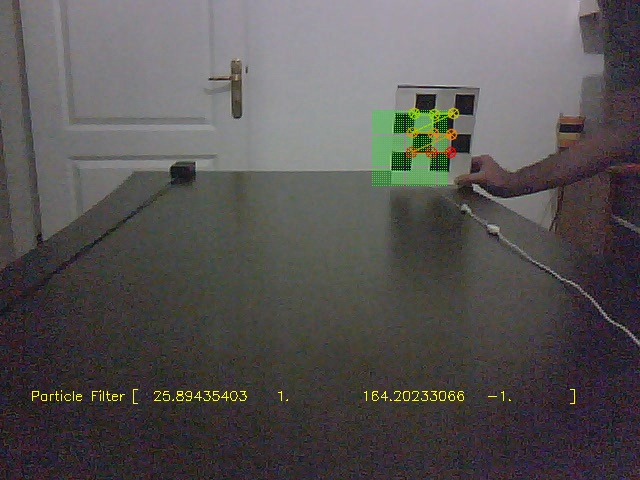
\includegraphics[height=4cm]{cb-pf-1.jpg}

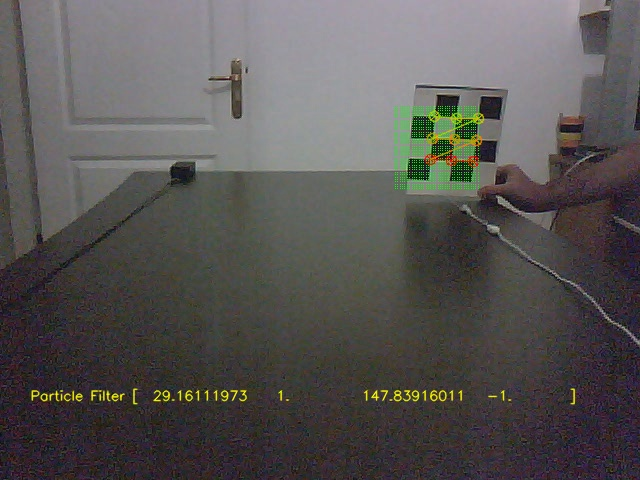
\includegraphics[height=4cm]{cb-pf-2.jpg}

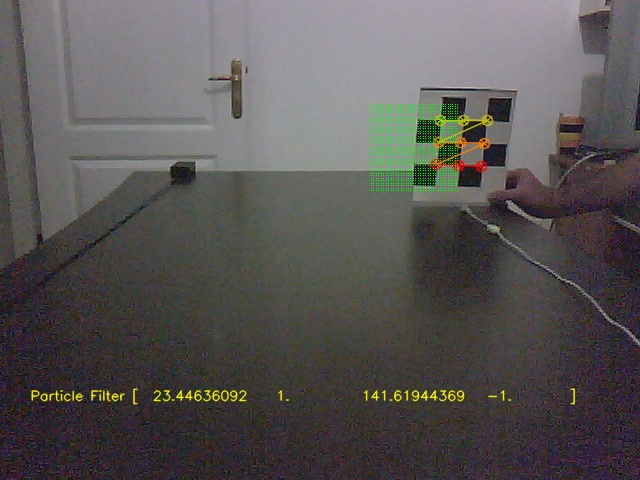
\includegraphics[height=4cm]{cb-pf-3.jpg}

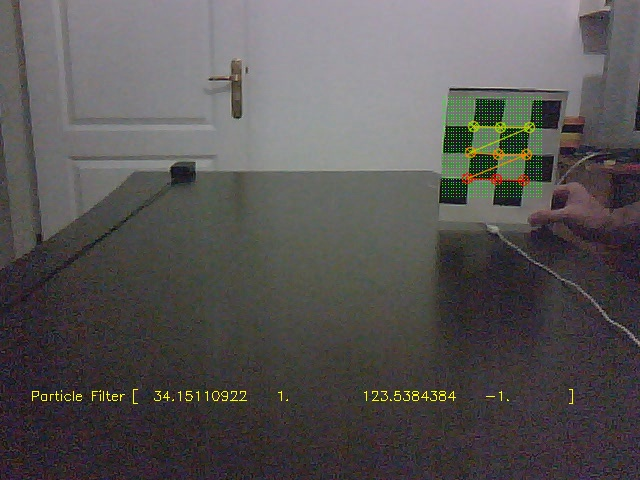
\includegraphics[height=4cm]{cb-pf-4.jpg}

Kaynaklar

http://dl.dropbox.com/u/1570604/skfiles/campy/chessb-left.avi

http://dl.dropbox.com/u/1570604/skfiles/campy/chessb-right.avi

S. Marsland, Machine Learning: An Algorithmic Perspective, CRC Press,
2009.

S. Thrun, W. Burgard, and D. Fox, Probabilistic Robotics, MIT Press,
Cambridge, MA, 2005

C. Bishop Pattern Recognition and Machine Learning , 2006.

Rabiner L. R. , A Tutorial on Hidden Markov Models and Selected
Applications in Speech Recognition, Proceedings of IEEE vol. 77, no. 2,
pp. 257-286, 1989.

Roweis S. and Z. Ghahramani, A Unifying Review of Linear Gaussian Models,
Neural Computation 11(2):305-345, 1999.

Ghahramani Z., H. E. Hinton, Parameter Estimation for Linear Dynamical
Systems, Technical Report CRG-TR-96-2

ftp://ftp.cs.toronto.edu/pub/zoubin/tr96-2.ps.gz], Department of Computer
Science, University of Toronto, 1996. 

Ghahramani Z., H. E. Hinton, Switching State Space Models, Technical Report
CRG-TR-96-3, Dept. Comp. Sci., Univ. Toronto, 1996. 

Shumway R., H. S. Stoffer Time series analysis and its applications 2nd
Edition, New York, Springer, (Springer texts in statistics), 2000. 

Jordan M. I. , C. Bishop An Introduction to Graphical Models, Not yet
published, 2000. 

Kalman R. E., A New Approach to Linear Filtering and Prediction Problems,
Transactions of the ASME-Journal of Basic Engineering, 82 (Series D):
35-45, 1960.

Kalman, R.E. and R.S. Bucy, New results in filtering and prediction theory,
Trans. ASME J. Basic Eng., 83, 95-108, 1961. 

Welling, M., The Kalman Filter - Lecture Tutorial, California Institute of
Technology, 2008. 

Lall, S., Modern Control 2 Lecture Notes, Stanford University, 2006.

Quantitative Economics Lecture Notebooks - thttp://quant-econ.net/kalman.html

\end{document}

